%% Supplementary material for the Objective 2 paper. Compile after main.tex:
%%   pdflatex main; pdflatex supplement; bibtex supplement; pdflatex supplement x2; pdflatex main
%% Numbers without the prefix S refer to the main paper (xr reads main.aux).
\documentclass[10pt,a4paper]{article}
\usepackage[T1]{fontenc}
\usepackage{lmodern}
\input{glyphtounicode}\pdfgentounicode=1
\usepackage[margin=2.3cm]{geometry}
\usepackage[authoryear]{natbib}
\usepackage{booktabs,multirow,xspace,adjustbox,graphicx,enumitem,amsmath}
\usepackage[table]{xcolor}
\usepackage[expansion=false]{microtype}
\usepackage{xr}\externaldocument{main}
\usepackage[hidelinks]{hyperref}
\newcommand{\pending}[1]{\textcolor{red!70!black}{[PENDING: #1]}}
\newcommand{\mono}{Mono-fix\xspace}
\newcommand{\poly}{Poly-fix\xspace}
\renewcommand{\thesection}{S\arabic{section}}
\renewcommand{\thetable}{S\arabic{table}}
\renewcommand{\thefigure}{S\arabic{figure}}
\setlength{\parskip}{3pt}
\title{Supplementary Material for\\``Mono-fix or Poly-fix? Bug Fixes Beyond the Main Language\\and Their Effect on Bug Localization''}
\author{A Eashaan Rao \and Sridhar Chimalakonda\\[2pt]\small Indian Institute of Technology Tirupati, India}
\date{}
\begin{document}
\maketitle
\noindent This supplement gives the tables and analyses that support the paper.
Sections, tables and figures numbered with the prefix S are in this
supplement; numbers without it refer to the paper.

\section{Related work: positioning}\label{app:related}

\begin{table*}[t]
\caption{Positioning: what each line of work provides and what this study adds.}
\label{tab:positioning}
\small
\begin{adjustbox}{max width=\linewidth}\begin{tabular}{p{3.3cm}p{6.2cm}p{6.6cm}}
\toprule
Line of work & Strength we use & Gap this study addresses \\
\midrule
Fix characterisation & Method for classifying fixes; multi-hunk taxonomy & Classifies by size and distance, not by file type \\
Cross-language BL (BLAZE, BeetleBox) & Multi-language ground truth; language-agnostic technique & Unit is a single-language fix within a project \\
Language-interaction bugs (xLoc) & Bugs at language boundaries & Bugs \emph{caused} by a boundary, not fixes that \emph{cross} one \\
Dataset quality & Ground truth affects measured performance & Concerns files wrongly included, not files fixes contain \\
Polyglot SE / RTS & Monolingual tools can be unsafe on polyglot code & Different task (testing, not localization) \\
LLM-based localization (agents, rankers) & Current techniques; graph-based tools; retrieve-and-rerank & Evaluated on source-only targets (SWE-bench, LocBench) \\
\bottomrule
\end{tabular}\end{adjustbox}
\end{table*}

\section{Study-design details}\label{app:design}

\paragraph{Classification protocol.} A fifth criterion (C5) decides only which
languages receive their own row in the statistics: at least 15 Poly-fix bugs
across at least two projects.
The written protocol was checked on a stratified sample of 50 bugs before any
technique was run: annotators classify every fix file (counted or excluded,
language, test scope) and every bug (label, keep, secondary languages,
sub-type) from the protocol alone, without access to the classifier; the
two-person agreement is reported in Section~\ref{sec:classification}. In
that round both annotators independently raised the same rule readings (closed dev-tooling list, \texttt{scripts/ci/} not being the CI
path \texttt{.ci/}, generated files outside \texttt{generated/}, module names
ending in \texttt{-testing}, tooling under \texttt{test/}); all were applied as
written. One annotator noticed that the rules document listed a
documentation-path rule that the protocol and the frozen code do not apply;
its wording was corrected, with no effect on any result, because files with a
documentation extension are excluded wherever they are. The protocol now also
states that \emph{counts} asks only whether a boundary rule excludes a file,
not whether the file caused the bug, the reading behind the four slips. Three
of the questioned rule readings were kept frozen rather than amended; amending
them would change the Poly-fix label of at most 1.4\% of Poly-fix bugs. Test scope is decided from the path, so test-harness code in a \texttt{test} package under \texttt{src/main/} counts as test (96 primary-language ground-truth files); this affects only S1 and the sub-type.

\paragraph{Bugs outside the primary-anchored set.} Of the 4{,}995 bugs of the
six projects, 1{,}401 are not primary-anchored: 417 change no counted file (documentation or changelog only), and 984---21.5\% of
the 4{,}578 bugs with counted fix files---change counted files but none in the
primary language: 520 single-language fixes in another language (mostly the
TypeScript and Vue front-end of dolphinscheduler), 374 fixes of configuration,
schema or build files only, and 90 multi-language fixes without the primary
language. These no-primary fixes cannot enter the Mono-fix/Poly-fix
comparison, but they are the case in which a parser-dependent technique can
reach no fixed file at all, so we analyse them as a separate group
(Section~\ref{sec:removed}). The 1{,}226 filter-excluded reports are distributed as elasticsearch 363,
airflow 383, ansible 295, dolphinscheduler 83, localstack 63 and liquibase 39.

\paragraph{Why Java and Python.} The restriction is by design, not for lack of data: BeetleBox has more C++ and JavaScript bugs (5{,}268 and 3{,}783) than Java or Python bugs (3{,}707 and 3{,}759). The pair also covers a statically and a dynamically typed ecosystem.

\paragraph{Departures from the original implementations.} Table~\ref{tab:deviations} lists every departure of our runs from the authors' code. FLIM has 19 IR features in the original and 18 in our runs.

% moved from main.tex to the supplementary material (2026-11-09)
\begin{table*}[t]
\caption{Departures from the original implementations.}
\label{tab:deviations}
\small
\begin{adjustbox}{max width=\linewidth}\begin{tabular}{p{1.8cm}p{14.3cm}}
\toprule
Technique & Departure and reason \\
\midrule
BLAZE & Hard examples are weighted inside the batch by the loss; the paper's GPT-mined hard-example set is BeetleBox-specific. Comments are not stripped before chunking. The learning rate is selected by validation MAP from $\{2{\times}10^{-7}, 2{\times}10^{-6}, 2{\times}10^{-5}\}$ (the paper's value and two larger ones), because the paper's value was set for $\sim$11{,}000 training bugs and our projects have 100--600. Selected in fold~1: $2{\times}10^{-7}$ for liquibase and localstack, $2{\times}10^{-6}$ for dolphinscheduler, $2{\times}10^{-5}$ for elasticsearch, ansible and airflow; all selected values in the learning-rate table of the replication package. \\
FLIM & Positive pairs are the functions the fix changed (diff overlap), not every function of the fixed file. Its TF-IDF features split identifiers at camel-case boundaries without keeping the whole identifier. The CodeSearchNet pairs of the paper's MIX set are not added. IR feature f2 (API-enriched similarity) needs JDK documentation and has no Python counterpart, so it is dropped. Other positives of the same report are masked out of the in-batch loss. The learning rate is selected by validation MAP between the two published values ($2{\times}10^{-5}$ in the released code, $5{\times}10^{-5}$ in the paper). Selected in fold~1: $2{\times}10^{-5}$ for elasticsearch and airflow, $5{\times}10^{-5}$ for the other four projects; the learning-rate table of the replication package. \\
LocAgent & No change to prompts, tools or search logic. One bug in its driver is fixed: a tool output is passed to \texttt{eval()}, which fell back to the raw text only on a syntax error, so outputs beginning with a path such as \texttt{lib/ansible/\ldots} raised a name error, killed the worker and left the run waiting forever; the fix extends the existing fallback to every error, so every output that did not crash is handled exactly as before. An adapter exports our test bugs as LocAgent instances (pre-fix commit, report text; the patch field is left empty) and builds LocAgent's graph and BM25 indexes from our local clones with LocAgent's own builders, materialising the full commit tree (not \texttt{git archive}, which drops paths marked \texttt{export-ignore}), so LocAgent sees the same pre-fix snapshot as the other techniques. We use the paper's fine-tuned 7B model rather than its 32B model: the 32B bf16 weights (65.5\,GB) exceed our 48\,GB GPU, and loading them with on-the-fly FP8 quantization ran out of memory. The paper reports both; its ablations use the 7B model (file-level Acc@5 on SWE-bench Lite 88.3 for 7B, 92.7 for 32B). \texttt{litellm} 1.52.1, pinned by LocAgent, is no longer on PyPI; 1.53.1 is used. \\
SweRank & No change to the corpus builder, retriever, prompts, reranking loop or permutation parsing; reranking uses the authors' sequential path, one bug at a time. An adapter feeds the same bugs, pre-fix snapshots and report text as for LocAgent, and maps the reranked functions to files by first appearance; files beyond the top 100 functions keep the retriever's order. SweRank's structure builder files a snapshot's top-level files under the repository name, which collides with a package directory of the same name (\texttt{localstack/}, \texttt{airflow/}); file paths are resolved against the snapshot. A function text already embedded for an earlier bug of the same project is not embedded again. vLLM's memory share is lowered from 0.9 to 0.55 for our shared GPU. We use the Small models (7B reranker), a configuration documented in the released code, rather than the Large ones: the 32B reranker exceeds our GPU, as for LocAgent. A faster variant that sent the reranking prompts of many bugs to the GPU together did not reproduce the sequential order (0 of 6 bugs) and was not used. \texttt{pyarrow}, which the authors do not pin, is set to 20.0.0. \\
\bottomrule
\end{tabular}\end{adjustbox}
\end{table*}


\paragraph{Techniques not run.} Of the other parser-based candidates, BL-GAN
\citep{zhu2022bl} represents an unparseable file by its path only and is
recorded in the feasibility analysis (Table~\ref{tab:feas}), but not run: its
behaviour on secondary files is fixed by its architecture, so running it would
add a second technique with the same reach as FLIM-strict, at the cost of a GAN
training per project and fold. TRANP-CNN \citep{huo2019deep} treats text lines
as statements without parsing and is therefore language-agnostic in our sense.
Agentless \citep{xia2024agentless} reads only Python files, as LocAgent does,
so it would not add a different reach, and its published configuration uses
GPT-4o, which cannot be run locally.

\paragraph{What LocAgent and SweRank index.} LocAgent's graph builder uses
Python's \texttt{ast}, and its BM25 index keeps only \texttt{.py} files outside
test directories; all four of its tools operate on these two indexes, so Python
test files are reachable through the graph but not through keyword search, and
no non-Python file is reachable. SweRank's corpus builder keeps the functions of
\texttt{.py} files whose path does not contain ``test''. SweRank's authors
describe existing ranking approaches, theirs included, as Python-centric, and
SweRank+ \citep{reddy2025sweranplus} was not released when we checked
(November 2026). Porting either parser to Java would make a new technique whose
result could not be separated from the Python-only training.

\paragraph{Test sets.} Fold~1 has 719 primary-anchored test bugs (483 Mono-fix, 213 Poly-fix and
23 that are multi-language only outside the broad grain); fold~2 has 718 (505,
206, 7). A bug whose fixed files were all added by the fix has nothing to rank
and is left out of the rank metrics.

\paragraph{File universe.} For each test bug, every technique scores every
file of the pre-fix snapshot that is text (at most 1\,MB and no NUL byte in
its first 8\,KB). The \emph{primary universe} R keeps the files that the
classification ruleset counts; the \emph{text universe} T keeps all text files
and is used for sensitivity. There is no retrieval stage that pre-selects
candidates. The median R is 1{,}890 (localstack) to 21{,}658 (elasticsearch)
files per snapshot.

\paragraph{Change set and class.} Besides the reasons given in
Section~\ref{sec:evaluation}, the class must be defined on the same files as
the target, or a bug could be Poly-fix by files that are never scored. LocAgent
and SweRank exclude test files by design, a further reason to report every
result also without test files in the ground truth (S1).

\paragraph{Metric details.} Top-$k$ is computed for $k\in\{1,5,10\}$. Ties are
resolved by expected rank under random tie-breaking, and for each bug we also
compute the RR and Top-10 that random ranking would reach given the number of
candidates and ground-truth files. AP@10 counts ranks beyond 10 as misses and
is still divided by the number of reachable ground-truth files, so a bug with
more than ten cannot reach 1; with it, complete-fix recall@10, Top-$k$ and
RR@10 are secondary. In the LocAgent trial a Poly-fix bug had RR 1.0 and AP
0.25: the Python file was ranked first, and the YAML and INI files of the fix
were never returned, the case that made AP the primary outcome. LocAgent and
SweRank are run on the 395 fold-1 and 395 fold-2 test bugs of the Python
projects, plus the filter-excluded bugs in those test windows (121 and 136).
The files SweRank cannot see are left unscored and share the last ranks;
counting them as misses instead, as the parseable view does for FLIM-strict,
gives the same class effect ($-0.172$ in both views).

\paragraph{Ablation and repeated runs.} To test whether a language-agnostic
technique's ranking of secondary files is limited by its training data, we
train BLAZE once more on chunks of \emph{all} fix files rather than only
project-language files (BLAZE-all; fold~1, seed 13, the learning rate selected
for BLAZE). LocAgent samples at temperature 1.0; we repeat it twice on a fixed
random subset of 100 fold-1 bugs to report run-to-run variation. SweRank
trains nothing and decodes greedily, so it is run once; because greedy
decoding on a GPU is not guaranteed to be bit-identical between runs, we re-run
it on a random subset of fold-1 bugs (20, plus one bug that differed in an
earlier check) to measure the variation.

\paragraph{Diagnostic variants: implementation.} In reciprocal rank fusion a
file at rank $r$ in its list scores $1/(60+r)$; the hybrids of FLIM-strict,
LocAgent and SweRank are built from the stored score files. The co-change
variant uses only commits made before the report, excluding merges, the fix
commit and commits that change more than 30 files, and scores every file $b$
the technique does not rank by $\sum_{a} c(a,b)/(n(a)\,r_a)$ over the
technique's top five files $a$, where $n(a)$ counts the commits that changed
$a$, $c(a,b)$ those that changed both, and $r_a$ is $a$'s rank; the two lists
are merged as for the hybrid. SweRank on all text files adds the non-Python
files, the Python test files and the Python files without a function as
50-line chunks in SweRank's document format (path, then text); a file's
position is that of its best document. The full technique is run on the
all-files corpus and on the non-Python-only corpus; the two other partial
corpora (Python test files only; all files with at most 10 chunks) are run with
the retriever only, and were added after the other variants. Each variant is
compared with the original technique and with BM25 on the same bugs by MAP over
all bugs and per class, by the paired tests and interaction models of RQ4, and
by the MAP of the secondary files with the other ground-truth files removed,
split into behaviour-bearing and test-asset files.

\paragraph{Training budget and hyper-parameters.} Every hyper-parameter comes
from the authors' released code except the learning rate. The neural
techniques are trained up to their papers' epoch counts (BLAZE 15, FLIM 10),
with the epoch selected on the validation split by each technique's own
criterion (BLAZE: validation loss; FLIM: validation MRR) and an early-stopping
patience of 3 epochs. The learning rate is chosen for both techniques by one
rule: validation MAP, the primary outcome, over a small grid around the
published values ($\{2{\times}10^{-7}, 2{\times}10^{-6}, 2{\times}10^{-5}\}$
for BLAZE, whose $2{\times}10^{-7}$ was set for about 11{,}000 bugs pooled
across projects; $\{2{\times}10^{-5}, 5{\times}10^{-5}\}$ for FLIM, the
values of its code and paper). We do not select on the training loss, which
measures how a report separates its own chunks from about twenty in-batch
chunks rather than how a file ranks among thousands; in our pilot the two
criteria disagreed. The choice is made once per project and fold with the
first seed; the test set is never used. BLAZE selected the published rate in
five of twelve project--folds, the middle rate in two and the largest in five,
where the validation loss was lowest after one to four epochs, so a larger
rate would only over-fit sooner (Table~\ref{tab:lr}, with epochs and GPU cost).

Each neural technique is run with seed 13 on every project and fold, and with
seeds 42 and 2027 on fold~1 of localstack, dolphinscheduler and liquibase.
Bootstrap intervals and paired tests account for which bugs are in the test
set, not for the randomness of training, which repeated runs measure
\citep{arcuri2011practical}. BM25 is deterministic and run once.

% generated by Scripts/analysis/paper_tables.py -- do not edit
\begin{table*}[t]
\caption{Learning rate selected on validation MAP (seed 13) and, in parentheses, the selected epoch / epochs run before early stopping (BLAZE at most 15, FLIM at most 10).}
\label{tab:lr}
\footnotesize
\begin{adjustbox}{max width=\linewidth}\begin{tabular}{lllll}
\toprule
 & \multicolumn{2}{c}{BLAZE} & \multicolumn{2}{c}{FLIM} \\
\cmidrule(lr){2-3}\cmidrule(lr){4-5}
Project & fold 1 & fold 2 & fold 1 & fold 2 \\
\midrule
elasticsearch (J) & $2{\times}10^{-5}$ (1/4) & $2{\times}10^{-5}$ (4/7) & $2{\times}10^{-5}$ (2/5) & $2{\times}10^{-5}$ (6/9) \\
liquibase (J) & $2{\times}10^{-7}$ (15/15) & $2{\times}10^{-6}$ (8/11) & $5{\times}10^{-5}$ (6/9) & $2{\times}10^{-5}$ (3/6) \\
dolphinscheduler (J) & $2{\times}10^{-6}$ (12/15) & $2{\times}10^{-7}$ (11/14) & $5{\times}10^{-5}$ (2/5) & $2{\times}10^{-5}$ (9/10) \\
ansible (P) & $2{\times}10^{-5}$ (1/4) & $2{\times}10^{-7}$ (12/15) & $5{\times}10^{-5}$ (3/6) & $5{\times}10^{-5}$ (5/8) \\
airflow (P) & $2{\times}10^{-5}$ (1/4) & $2{\times}10^{-5}$ (1/4) & $2{\times}10^{-5}$ (3/6) & $2{\times}10^{-5}$ (6/9) \\
localstack (P) & $2{\times}10^{-7}$ (14/15) & $2{\times}10^{-7}$ (15/15) & $5{\times}10^{-5}$ (2/5) & $2{\times}10^{-5}$ (7/10) \\
\bottomrule
\end{tabular}\end{adjustbox}
\\[2pt]{\footnotesize Training and scoring cost on one NVIDIA L40 (all seeds): BLAZE: 18 runs, 74 GPU-hours; BLAZE-all: 6 runs, 13 GPU-hours; FLIM: 18 runs, 14 GPU-hours.}
\end{table*}


\paragraph{Statistical details.} $n_{\mathrm{gt}}$ is included because Poly-fix bugs have more ground-truth
files and Top-$k$ is easier with more targets. If the random-intercept model
cannot be fitted, we fall back to project fixed effects with HC3 standard
errors; with six projects, cluster-robust errors are not used (the fallback was
needed for 49 of 832 class-effect models and 97 of 380 interaction models,
never for a main AP analysis except the SweRank reranker comparison). A logistic
model on Top-10 with project fixed effects is the robustness check. The two
folds are pooled with fold as a fixed effect. Because
$n_{\mathrm{gt}}$ differs strongly between the classes (4.3 against 2.4
reachable files on average), we also compare the classes within strata of
equal $n_{\mathrm{gt}}$ (1, 2, 3, 4, 5 or more), weighting each stratum by its
size, with a bootstrap interval. The false-discovery rate is controlled separately over all class-effect tests (832) and all interaction tests (380). LocAgent
is compared with BM25 on the Python projects with the same paired tests on
AP@10 (secondary: complete-fix recall@10, Top-10, RR@10), and SweRank on the
same bugs on AP (secondary: complete-fix recall@10, RR, Top-10). Comparing
SweRank with its own retriever separates what the LLM reranker contributes
from what the candidate set allows. Because
AP is bounded and has a mass at 0, we refitted the class-effect and
interaction models as fractional-logit regressions with project fixed
effects. The average marginal effects agree with the linear estimates (BM25
$-0.026$, BLAZE $-0.016$, FLIM-strict $-0.132$, LocAgent $-0.158$, SweRank
$-0.172$, SweRank on all files $-0.045$), each is significant exactly where the
linear one is, and every interaction keeps its sign and significance (the
parseable-view control: $p=0.95$). The statistics have further known limits: bootstrap intervals resample bugs and ignore correlation within a project over time, and bugs with several seeds enter the models as seed averages next to single-seed bugs.

\section{RQ1 details}\label{app:rq1}

Over all 4{,}995 bugs, including those whose fix changes no file in the primary language, the broad-grain share is 19.7\%. Every counted secondary file in the Poly-fix bugs is also in the dataset's ground truth (Table~\ref{tab:secondary}). The behaviour-bearing secondary files are mostly YAML (147
bugs), XML (88), JSON (51), TypeScript (47), JavaScript (41), INI (30), Shell
(25) and Gradle (21). By project, test-asset-only bugs make up 91.9\% of the Poly-fix bugs of ansible, 85.9\% of liquibase, 83.2\% of localstack and 70.3\% of elasticsearch, but 0.6\% of airflow and of dolphinscheduler.

Table~\ref{tab:sensitivity} reports how the broad-grain prevalence changes
when one boundary rule is changed at a time. Excluding test files reduces it
to 11.0\% and counting changelog fragments raises it to 41.3\%; counting
documentation or deletions changes it by at most 0.1 percentage points.
Restricting to programming languages gives the strict grain, 8.2\%.

Among the 1{,}226 bugs BeetleBox removed because their report names a fixed
file, 1{,}055 would be kept, and 15.9\% of those are Poly-fix at the
broad grain, against 27.4\% of the primary-anchored bugs; the share is lower in five of
the six projects (liquibase: 50.0\% against 49.7\%). Counting the filter-excluded bugs
as well gives 24.8\% (1{,}153 of 4{,}649). The dataset's filter therefore
raised the Poly-fix share of the primary-anchored set by 2.6 percentage points.

% moved from main.tex to the supplementary material (2026-11-09)
\begin{table}[t]
\caption{Secondary languages in Poly-fix bugs (primary-anchored bugs containing at least one such file).}
\label{tab:secondary}
\small
\begin{adjustbox}{max width=\linewidth}\begin{tabular}{lrr}
\toprule
Secondary language & Poly-fix bugs & Projects \\
\midrule
YAML & 497 & 6 \\
JSON & 163 & 6 \\
XML & 117 & 4 \\
Shell & 101 & 5 \\
Groovy & 72 & 2 \\
TypeScript & 47 & 2 \\
JavaScript & 43 & 3 \\
Gradle & 33 & 1 \\
SQL & 19 & 2 \\
17 further languages & 1--19 each & 1--3 \\
\bottomrule
\end{tabular}\end{adjustbox}
\end{table}

% moved from main.tex to the supplementary material (2026-11-09)
\begin{table}[t]
\caption{Sensitivity of Poly-fix prevalence (broad grain, share of primary-anchored bugs) to the boundary rules, one rule changed at a time.}
\label{tab:sensitivity}
\small
\begin{adjustbox}{max width=\linewidth}\begin{tabular}{lrr}
\toprule
Rule change & Poly-fix & \% \\
\midrule
None (default rules) & 985 & 27.4 \\
Only programming languages count & 294 & 8.2 \\
Exclude test files$^{a}$ & 365 & 11.0 \\
Count changelog fragments & 1{,}484 & 41.3 \\
Count documentation & 985 & 27.4 \\
Count deletions$^{b}$ & 989 & 27.5 \\
\bottomrule
\end{tabular}\end{adjustbox}
\\[2pt]{\footnotesize $^{a}$3{,}324 primary-anchored bugs under this rule. $^{b}$3{,}595 primary-anchored bugs. Merging data-configuration languages into one pseudo-language is a label-level check only (label-level prevalence unchanged at 28.7\%); it is not defined for the grains.}
\end{table}


\paragraph{Beyond the six projects.} To see how far the selection shapes these
figures, we classified the bugs of all 13 Java and Python projects of BeetleBox
with at least 100 reports in the same way (Table~\ref{tab:rq1all}). Re-running
the procedure on the six study projects reproduces the main classification for
all 4{,}995 bugs. The selection effect is the difference between the study
projects and the seven others, and it is substantial. Of the primary-anchored
bugs, 27.4\% are Poly-fix at the broad grain in the study projects against
18.5\% in the others (per-project medians 29.0\% and 17.5\%), and 21.0\%
against 8.5\% at the data-format grain. Only the strict grain is higher in
the others (10.6\% against 8.2\%), and this comes from two projects. The others
also differ in a second respect: only 35.7\% of their bugs with a counted
fix file are primary-anchored, against 78.5\% in the study projects. Counted
over all bugs with a counted fix file, broad-grain Poly-fix bugs are 21.5\% of
the study projects' bugs and 6.6\% of the others'.

Two of the seven are cases where a single primary language does not describe
the project. In ccxt only 40 of 674 bugs with counted files touch Python, and
in posthog 101 of 382; most of their fixes are in other languages. Their high
shares at the broad and strict grains (70.0\% and 36.6\% broad) describe these
small subsets, not the projects. Without them, the five remaining projects have
a broad-grain share of 12.8\% and a strict share of 4.1\% of 680
primary-anchored bugs. The proxy predicts prevalence only loosely (dubbo:
proxy 7.4\%, prevalence 7.5\%; openrefine, 29.4\% and 22.8\%).
Pooling all 13 projects gives 25.8\%, but 81\% of that pool are the study
projects' bugs, so it is not an independent estimate. Our prevalence figures
therefore describe projects selected to contain both classes and are upper
values for BeetleBox as a whole.

\begin{table}[t]
\caption{Poly-fix prevalence over all 13 Java and Python projects of BeetleBox with at least 100 bug reports (ruleset 0.2.0), the six study projects and the seven others.}
\label{tab:rq1all}
\small
\setlength{\tabcolsep}{3pt}
\begin{adjustbox}{max width=\linewidth}\begin{tabular}{lrrrrrrrr}
\toprule
 & & & & & \multicolumn{3}{c}{\% of anchored} & \% of cnt. \\
\cmidrule(lr){6-8}\cmidrule(lr){9-9}
Project & Bugs & Anch. & Anch.\,\% & Proxy & broad & data & strict & broad \\
\midrule
\multicolumn{9}{l}{\emph{Study projects}} \\
dolphinscheduler (J) & 1{,}363 & 698 & 53.6 & 29.4 & 23.6 & 14.6 & 10.7 & 12.7 \\
elasticsearch (J) & 970 & 721 & 84.8 & 49.4 & 17.8 & 15.1 & 0.3 & 15.1 \\
liquibase (J) & 241 & 199 & 84.7 & 42.7 & 49.7 & 20.1 & 35.7 & 42.1 \\
airflow (P) & 1{,}181 & 917 & 85.2 & 32.9 & 18.8 & 14.2 & 5.5 & 16.0 \\
ansible (P) & 768 & 626 & 94.7 & 66.0 & 43.5 & 39.1 & 13.4 & 41.1 \\
localstack (P) & 472 & 433 & 95.6 & 37.1 & 34.4 & 29.6 & 2.8 & 32.9 \\
\quad pooled & 4{,}995 & 3{,}594 & 78.5 & 41.1 & 27.4 & 21.0 & 8.2 & 21.5 \\
\midrule
\multicolumn{9}{l}{\emph{Other eligible projects}} \\
dubbo (J) & 379 & 253 & 67.8 & 7.4 & 7.5 & 5.5 & 0.0 & 5.1 \\
openrefine (J) & 620 & 189 & 34.9 & 29.4 & 22.8 & 16.9 & 13.8 & 7.9 \\
selenium (J) & 134 & 46 & 46.0 & 11.9 & 2.2 & 0.0 & 2.2 & 1.0 \\
ccxt (P) & 690 & 40 & 5.9 & 11.8 & 70.0 & 10.0 & 67.5 & 4.2 \\
langchain (P) & 130 & 112 & 97.4 & 26.2 & 8.9 & 2.7 & 0.0 & 8.7 \\
odoo (P) & 115 & 80 & 70.8 & 12.2 & 17.5 & 16.2 & 1.2 & 12.4 \\
posthog (P) & 403 & 101 & 26.4 & 48.6 & 36.6 & 4.0 & 31.7 & 9.7 \\
\quad pooled & 2{,}471 & 821 & 35.7 & 22.3 & 18.5 & 8.5 & 10.6 & 6.6 \\
\midrule
All 13 & 7{,}466 & 4{,}415 & 64.2 & 34.9 & 25.8 & 18.7 & 8.6 & 16.5 \\
\bottomrule
\end{tabular}\end{adjustbox}
\\[2pt]{\footnotesize Anch.: primary-anchored bugs; Anch.\,\%: their share of the bugs with a counted fix file. Proxy: share of fixes whose changed files have more than one extension (pooled: weighted by bugs). Prevalence in \% of primary-anchored bugs (``data'': data-format grain) and, in the last column, broad-grain Poly-fix bugs in \% of all bugs with a counted fix file. In ccxt and posthog fewer than a third of the bugs touch the assigned primary language, so their prevalence describes a small subset. The study projects re-classified by the same script agree with the main classification for all 4{,}995 bugs.}
\end{table}


\section{RQ2--RQ4 details}\label{app:rq234}

\paragraph{Reachability.} Table~\ref{tab:reach} gives the reachability of the
ground-truth files in both folds before any technique is run. Of the 984
no-primary fixes, 138 fall into the fold-1 test periods and 149 into the
fold-2 test periods. SweRank's corpus contains 95.6\% (Mono-fix) and 94.3\%
(Poly-fix) of the primary-language non-test ground-truth files, no test file
and no file in another language. In fold~1 the unparseable ground-truth files
of Poly-fix test bugs are YAML (108), JSON (70), TypeScript (35), Shell (22),
XML (17), Groovy (9), SQL (7) and others; none has status
\texttt{parse\_error}, which largely follows from criterion C2 but would
otherwise have pointed to our tooling.

\begin{table}[t]
\caption{Reachability of ground-truth files in the test sets, before any technique is run (fold~1; fold~2 in parentheses).}
\label{tab:reach}
\small
\setlength{\tabcolsep}{3pt}
\begin{adjustbox}{max width=\linewidth}\begin{tabular}{lrr}
\toprule
 & Mono-fix & Poly-fix \\
\midrule
Test bugs & 483 (505) & 213 (206) \\
Ground-truth files per bug, mean & 2.3 (2.5) & 4.4 (4.2) \\
Bugs with an added (unreachable) file & 8.7\% (7.7\%) & 34.7\% (33.0\%) \\
GT files parseable & 99.9\% (100\%) & 62.8\% (65.8\%) \\
Bugs with $\ge$1 parseable GT file & 100\% (100\%) & 98.1\% (98.5\%) \\
Bugs with only parseable GT files & 99.8\% (100\%) & 10.8\% (10.2\%) \\
\bottomrule
\end{tabular}\end{adjustbox}
\end{table}

\paragraph{RQ3: tables.} Tables~\ref{tab:rq3py}--\ref{tab:decomp} give the
results of the two LLM-based techniques per Python project, the adjusted class
effects for every outcome, and the decomposition including MRR.

\paragraph{RQ3 per project.} FLIM-strict ranks Poly-fix bugs lower in all three
Java projects (Cliff's $\delta$ from $-0.23$ to $-0.33$, Holm-adjusted
$p<0.05$). Per project, only BLAZE on dolphinscheduler differs significantly.
BM25's raw MAP falls from 0.311 to 0.274, most in ansible (0.401 to 0.245).
SweRank ranks Poly-fix bugs lower in all three Python projects (Cliff's
$\delta$ $-0.40$ in ansible and $-0.53$ in airflow, both significant; $-0.17$
in localstack). The effect is the same in both folds (FLIM-strict $-0.127$ and
$-0.135$; SweRank $-0.201$ and $-0.137$; Table~\ref{tab:sens}).

\paragraph{Decomposition.} On the primary-language files the Poly-fix and
Mono-fix MAPs are: BM25 0.291 against 0.311 (difference $[-0.056, 0.018]$),
FLIM-strict 0.395 against 0.370 ($[-0.017, 0.065]$), LocAgent 0.432 against
0.456 ($[-0.076, 0.028]$) and SweRank 0.468 against 0.477 ($[-0.058,
0.040]$). On the secondary files, random ranking would reach an MRR below
0.01.

\paragraph{localstack.} In localstack Poly-fix bugs score higher than Mono-fix
bugs for BM25 and BLAZE. 83\% of its Poly-fix bugs are test-asset-only, and 99
of its 149 Poly-fix fixes change a recorded snapshot file
(\texttt{*.snapshot.json}), stored next to the Python test module that records
it and keyed by that test's identifiers. Lexical and embedding similarity reach
these files through the same terms as the test.

\paragraph{BLAZE-all.} BLAZE-all, trained on chunks of all fix files instead of
primary-language files only, has the same class effect as BLAZE ($-0.031$;
interaction with BLAZE 0.001 $[-0.046, 0.048]$). At the size of within-project
training sets, BLAZE's ranking of secondary files is not limited by not having
seen them in training.

\paragraph{SweRank's reranker.} SweRank's retrieval stage has the same adjusted
class effect as the full technique ($-0.172$; MAP 0.415 and 0.227); the
reranker raises MAP by 0.062 on Mono-fix and by 0.050 on Poly-fix bugs, and the
two gains are equivalent within $\pm0.03$ (difference $0.001$
$[-0.025, 0.028]$, TOST $p = 0.017$).

% generated by Scripts/analysis/paper_tables.py -- do not edit
\begin{table*}[t]
\caption{RQ3 for the two techniques built on language models, which run on the Python projects only: MAP (AP@10 for LocAgent) of Mono-fix and Poly-fix test bugs per project (both folds) and Cliff's $\delta$ of Poly-fix against Mono-fix ($^{*}$: Holm-adjusted Mann--Whitney $p<0.05$). BM25 on the same bugs for reference. The last row is the adjusted class effect as in Section~\ref{sec:analysis}.}
\label{tab:rq3py}
\footnotesize
\setlength{\tabcolsep}{2.6pt}
\begin{adjustbox}{max width=\linewidth}\begin{tabular}{lr rrr rrr rrr rrr}
\toprule
 & & \multicolumn{3}{c}{BM25} & \multicolumn{3}{c}{LocAgent (AP@10)} & \multicolumn{3}{c}{SweRank} & \multicolumn{3}{c}{SweRank, retriever only} \\
\cmidrule(lr){3-5}\cmidrule(lr){6-8}\cmidrule(lr){9-11}\cmidrule(lr){12-14}
Project & $n$ M/P & Mono & Poly & $\delta$ & Mono & Poly & $\delta$ & Mono & Poly & $\delta$ & Mono & Poly & $\delta$ \\
\midrule
ansible (P) & 127/121 & .401 & .245 & $-$.18 & .606 & .334 & $-$.37$^{*}$ & .624 & .336 & $-$.40$^{*}$ & .557 & .282 & $-$.34$^{*}$ \\
airflow (P) & 305/55 & .353 & .352 & +.07 & .428 & .173 & $-$.56$^{*}$ & .442 & .193 & $-$.53$^{*}$ & .377 & .155 & $-$.51$^{*}$ \\
localstack (P) & 78/95 & .349 & .395 & +.13 & .324 & .196 & $-$.16 & .380 & .252 & $-$.17 & .336 & .199 & $-$.17 \\
\midrule
All (pooled) &  & .364 & .319 &  & .456 & .253 &  & .477 & .277 &  & .415 & .227 &  \\
Adjusted class effect &  & \multicolumn{3}{c}{$-$.030} & \multicolumn{3}{c}{$-$.163$^{*}$} & \multicolumn{3}{c}{$-$.172$^{*}$} & \multicolumn{3}{c}{$-$.172$^{*}$} \\
\bottomrule
\end{tabular}\end{adjustbox}
\end{table*}

% generated by Scripts/analysis/paper_tables.py -- do not edit
\begin{table*}[t]
\caption{RQ3: pooled class effect (Poly-fix minus Mono-fix) per technique, adjusted for $n_{\mathrm{gt}}$, $\log n_{\mathrm{cand}}$, report length, fold and project (linear mixed model, project random intercept; project fixed effects with HC3 errors where the mixed model did not converge). 95\% confidence intervals; $^{*}$: interval excludes 0.}
\label{tab:rq3models}
\footnotesize
\begin{adjustbox}{max width=\linewidth}\begin{tabular}{lrllll}
\toprule
Technique (view) & Bugs & AP & Complete-fix recall@10 & RR & Top-10 \\
\midrule
BM25, all files & 1399 & $-$.026 [$-$.068, +.016] & $-$.020 [$-$.073, +.033] & +.009 [$-$.043, +.061] & +.040 [$-$.022, +.101] \\
BM25, parseable & 1399 & $-$.129$^{*}$ [$-$.171, $-$.087] & $-$.157$^{*}$ [$-$.207, $-$.106] & $-$.050 [$-$.104, +.004] & $-$.051 [$-$.112, +.009] \\
FLIM-strict & 1399 & $-$.134$^{*}$ [$-$.174, $-$.093] & $-$.178$^{*}$ [$-$.227, $-$.129] & $-$.033 [$-$.086, +.020] & $-$.067$^{*}$ [$-$.123, $-$.010] \\
FLIM-fallback & 1399 & $-$.103$^{*}$ [$-$.145, $-$.062] & $-$.136$^{*}$ [$-$.186, $-$.086] & $-$.027 [$-$.080, +.026] & $-$.053 [$-$.110, +.005] \\
BLAZE & 1399 & $-$.021 [$-$.059, +.017] & $-$.010 [$-$.063, +.043] & +.012 [$-$.038, +.061] & +.029 [$-$.034, +.092] \\
BLAZE-all$^{a}$ & 691 & $-$.031 [$-$.085, +.024] & $-$.060 [$-$.135, +.014] & +.005 [$-$.095, +.105] & $-$.049 [$-$.140, +.041] \\
LocAgent$^{b}$ & 781 & $-$.163$^{*}$ [$-$.211, $-$.115] & $-$.185$^{*}$ [$-$.236, $-$.135] & $-$.053 [$-$.123, +.017] & $-$.057 [$-$.124, +.010] \\
SweRank$^{c}$ & 781 & $-$.172$^{*}$ [$-$.222, $-$.122] & $-$.190$^{*}$ [$-$.239, $-$.141] & $-$.040 [$-$.111, +.031] & $-$.029 [$-$.092, +.035] \\
SweRank, retriever only$^{c}$ & 781 & $-$.172$^{*}$ [$-$.220, $-$.125] & $-$.192$^{*}$ [$-$.242, $-$.142] & $-$.072$^{*}$ [$-$.143, $-$.001] & $-$.050 [$-$.119, +.019] \\
\bottomrule
\end{tabular}\end{adjustbox}
\\[2pt]{\footnotesize $^{a}$Fold 1 only. $^{b}$Python projects; AP@10 and RR@10, because LocAgent returns at most ten files. $^{c}$Python projects; full ranking of the files SweRank can see.}
\end{table*}

% generated by Scripts/analysis/paper_tables.py -- do not edit
\begin{table}[pos=t]
\caption{Where the Poly-fix penalty comes from (both folds). MRR of Mono-fix and Poly-fix bugs; MAP of Mono-fix bugs and of the primary-language and the secondary-language ground-truth files of Poly-fix bugs, each subset ranked with the other ground-truth files of the bug removed (the convention of Figure~\ref{fig:decomp}).}
\label{tab:decomp}
\footnotesize
\setlength{\tabcolsep}{2.4pt}
\begin{adjustbox}{max width=\linewidth}\begin{tabular}{lrrrrr}
\toprule
 & \multicolumn{2}{c}{MRR} & & \multicolumn{2}{c}{MAP, Poly-fix} \\
\cmidrule(lr){2-3}\cmidrule(lr){5-6}
Technique & Mono & Poly & MAP Mono & primary & secondary \\
\midrule
BM25 & .389 & .436 & .311 & .291 & .203 \\
FLIM-strict & .466 & .513 & .370 & .395 & n/a \\
FLIM-fallback & .462 & .511 & .365 & .383 & .055 \\
BLAZE & .329 & .396 & .255 & .286 & .142 \\
LocAgent$^{a}$ & .687 & .635 & .456 & .432 & .000 \\
SweRank$^{b}$ & .714 & .686 & .477 & .468 & .001 \\
SweRank, retriever only$^{b}$ & .630 & .570 & .415 & .389 & .001 \\
Random ranking & .004 & .009 &  &  &  \\
\bottomrule
\end{tabular}\end{adjustbox}
\\[2pt]{\footnotesize $^{a}$Python projects, AP@10 and RR@10. $^{b}$Python projects.}
\end{table}


\paragraph{RQ4: BM25 against FLIM.} Per project (Table~\ref{tab:rq4project}),
FLIM-strict leads on Mono-fix bugs in all six projects (significant in five),
and BM25 matches or exceeds it on Poly-fix bugs in five, significantly in
airflow ($+0.123$); ansible is the exception ($-0.024$). With the text
fallback, FLIM-fallback and BM25 are level on Poly-fix bugs ($+0.002$;
interaction $+0.079$). Top-10 shows a narrowing of FLIM's lead (interaction
$+0.096$ $[0.030, 0.162]$) without a reversal.

\paragraph{RQ4: BM25 against LocAgent.} BM25's AP@10 is 0.342 on Mono-fix bugs
(its MAP on these bugs is 0.364). Complete-fix recall@10 shows the same
interaction ($+0.147$). LocAgent leads on RR@10 in both classes, and its lead
narrows on Poly-fix bugs (interaction $+0.097$ $[0.016, 0.178]$) without
reversing. Per project the pattern holds in airflow and localstack, where BM25
leads on Poly-fix bugs by 0.149 and 0.160; in ansible LocAgent leads in both
classes, by less on Poly-fix ($-0.112$) than on Mono-fix bugs ($-0.218$). The
interaction is carried by behaviour-bearing Poly-fix bugs ($+0.182$; BM25 ahead
by 0.127), is present on test-asset-only bugs ($+0.092$), and is not
distinguishable from 0 without test files in the ground truth ($+0.062$
$[-0.005, 0.129]$), at the strict grain, or in fold~2 alone
(Figure~\ref{fig:sens}).

\paragraph{RQ4: BM25 against SweRank.} BM25's advantage on Poly-fix bugs,
0.042, is fragile: its bootstrap interval barely excludes 0
($[0.002, 0.082]$), the Wilcoxon test is not significant, and equivalence
cannot be shown (TOST $p=0.34$). Complete-fix recall@10 shows the same
interaction ($+0.151$), and SweRank leads on RR by 0.264 and 0.187
(interaction $+0.084$ $[0.004, 0.163]$). Per project
(Table~\ref{tab:rq4project}), BM25 leads on the Poly-fix bugs of airflow
($+0.159$) and localstack ($+0.143$), both significant; in ansible SweRank leads
in both classes, by less on Poly-fix ($-0.091$) than on Mono-fix bugs
($-0.223$). Unlike LocAgent's, the interaction excludes 0 in each fold
separately ($+0.172$ and $+0.113$), on behaviour-bearing ($+0.177$) and
test-asset-only Poly-fix bugs ($+0.097$); like LocAgent's, it is not
distinguishable from 0 without test files in the ground truth ($+0.061$), at the
strict grain or on the filter-excluded bugs (Figure~\ref{fig:sens}).

% generated by Scripts/analysis/paper_tables.py -- do not edit
\begin{table}[t]
\caption{RQ4 per project: mean paired difference BM25 $-$ FLIM-strict (AP), BM25 $-$ LocAgent (AP@10) and BM25 $-$ SweRank (AP) by class, both folds. $^{*}$: Holm-adjusted Wilcoxon signed-rank $p<0.05$.}
\label{tab:rq4project}
\footnotesize
\setlength{\tabcolsep}{3pt}
\begin{adjustbox}{max width=\linewidth}\begin{tabular}{lrrrrrr}
\toprule
 & \multicolumn{2}{c}{vs FLIM-strict} & \multicolumn{2}{c}{vs LocAgent} & \multicolumn{2}{c}{vs SweRank} \\
\cmidrule(lr){2-3}\cmidrule(lr){4-5}\cmidrule(lr){6-7}
Project & Mono & Poly & Mono & Poly & Mono & Poly \\
\midrule
elasticsearch (J) & $-$.013 & +.058 & -- & -- & -- & -- \\
liquibase (J) & $-$.084$^{*}$ & +.011 & -- & -- & -- & -- \\
dolphinscheduler (J) & $-$.069$^{*}$ & +.017 & -- & -- & -- & -- \\
ansible (P) & $-$.091$^{*}$ & $-$.024 & $-$.218$^{*}$ & $-$.112$^{*}$ & $-$.223$^{*}$ & $-$.091$^{*}$ \\
airflow (P) & $-$.066$^{*}$ & +.123$^{*}$ & $-$.101$^{*}$ & +.149$^{*}$ & $-$.088$^{*}$ & +.159$^{*}$ \\
localstack (P) & $-$.056$^{*}$ & +.040 & +.001 & +.160$^{*}$ & $-$.030 & +.143$^{*}$ \\
\bottomrule
\end{tabular}\end{adjustbox}
\end{table}


\paragraph{Sensitivity.} Figure~\ref{fig:sens} shows the RQ4 interaction under each condition, and
Table~\ref{tab:sens} also the RQ3 class effects. The FLIM-strict penalty and the BM25--FLIM-strict interaction
keep their sign and exclude 0 under every condition except the filter-excluded bugs,
whose Poly-fix sample is small. They are almost unchanged under the data-format
grain, the text universe T, the removal of merge commits and in each fold
separately; they are larger for behaviour-bearing Poly-fix bugs and smaller,
but still present, without test files. The control interaction includes 0
under every condition. The BM25--LocAgent interaction excludes 0 in the main
analysis and under most conditions, but not without test files, at the strict
grain or in fold~2 alone, where LocAgent's lead on Mono-fix bugs narrows on
Poly-fix bugs without reversing. The BM25--SweRank interaction behaves the
same way except in fold~2, where it excludes 0; SweRank's class effect
excludes 0 under every condition.

% generated by Scripts/analysis/paper_tables.py -- do not edit
\begin{table*}[t]
\caption{Robustness: RQ3 class effect and RQ4 interaction by Poly-fix sub-type and under each condition R1--R6 (AP; AP@10 for LocAgent; LocAgent and SweRank on the Python projects). $^{*}$: 95\% CI excludes 0. R6 uses the bugs BeetleBox removed because their report names a fixed file, scored by models trained on the primary-anchored bugs.}
\label{tab:sens}
\footnotesize
\setlength{\tabcolsep}{3pt}
\begin{adjustbox}{max width=\linewidth}\begin{tabular}{lrrrrrrrrr}
\toprule
 & \multicolumn{4}{c}{RQ3 class effect} & \multicolumn{5}{c}{RQ4 interaction (BM25 $-$ X)} \\
\cmidrule(lr){2-5}\cmidrule(lr){6-10}
Condition & BM25 & FLIM-strict & LocAgent & SweRank & FLIM-strict & FLIM-fallback & control & LocAgent & SweRank \\
\midrule
Main analysis & $-$.026 & $-$.134$^{*}$ & $-$.163$^{*}$ & $-$.172$^{*}$ & +.107$^{*}$ & +.079$^{*}$ & +.004 & +.137$^{*}$ & +.143$^{*}$ \\
Poly-fix: behaviour-bearing only & $-$.012 & $-$.155$^{*}$ & $-$.168$^{*}$ & $-$.169$^{*}$ & +.138$^{*}$ & +.111$^{*}$ & +.018 & +.182$^{*}$ & +.177$^{*}$ \\
Poly-fix: test-asset only & $-$.034 & $-$.113$^{*}$ & $-$.139$^{*}$ & $-$.147$^{*}$ & +.091$^{*}$ & +.061$^{*}$ & $-$.004 & +.092$^{*}$ & +.097$^{*}$ \\
R1 ground truth without tests & $-$.032 & $-$.080$^{*}$ & $-$.100$^{*}$ & $-$.094$^{*}$ & +.047$^{*}$ & +.043$^{*}$ & +.009 & +.062 & +.061 \\
R2 data-format grain & $-$.018 & $-$.126$^{*}$ & $-$.160$^{*}$ & $-$.165$^{*}$ & +.111$^{*}$ & +.076$^{*}$ & $-$.002 & +.148$^{*}$ & +.151$^{*}$ \\
R2 strict grain & $-$.100$^{*}$ & $-$.202$^{*}$ & $-$.207$^{*}$ & $-$.212$^{*}$ & +.096$^{*}$ & +.077$^{*}$ & +.033 & +.028 & +.037 \\
R3 text universe T & $-$.028 & $-$.133$^{*}$ & $-$.163$^{*}$ & $-$.172$^{*}$ & +.106$^{*}$ & +.079$^{*}$ & +.004 & +.140$^{*}$ & +.147$^{*}$ \\
R4 merge commits removed & $-$.026 & $-$.134$^{*}$ & $-$.163$^{*}$ & $-$.172$^{*}$ & +.108$^{*}$ & +.079$^{*}$ & +.005 & +.137$^{*}$ & +.143$^{*}$ \\
R5 fold 1 only & $-$.019 & $-$.127$^{*}$ & $-$.239$^{*}$ & $-$.201$^{*}$ & +.108$^{*}$ & +.075$^{*}$ & $-$.024 & +.210$^{*}$ & +.172$^{*}$ \\
R5 fold 2 only & $-$.031 & $-$.135$^{*}$ & $-$.085$^{*}$ & $-$.137$^{*}$ & +.106$^{*}$ & +.083$^{*}$ & +.028 & +.064 & +.113$^{*}$ \\
R6 filter-excluded bugs only & $-$.052 & $-$.125$^{*}$ & $-$.211$^{*}$ & $-$.158$^{*}$ & +.080 & +.029 & $-$.030 & +.154$^{*}$ & +.095 \\
\bottomrule
\end{tabular}\end{adjustbox}
\end{table*}


\begin{figure*}[t]
\centering
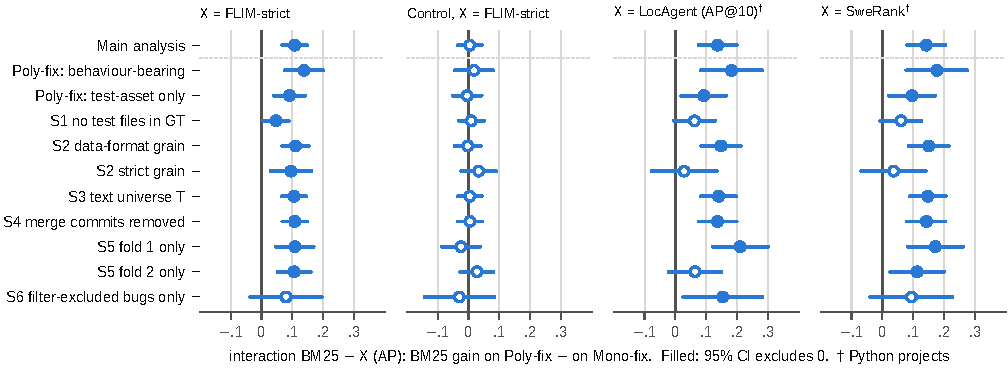
\includegraphics[width=\textwidth]{figures/fig_sensitivity.pdf}
\caption{RQ4 interaction (BM25's gain over technique X on Poly-fix bugs minus its gain on Mono-fix bugs, AP) under each sensitivity condition, with 95\% confidence intervals. The control compares BM25 restricted to parseable files with FLIM-strict. The RQ3 class effects under the same conditions are in Table~\ref{tab:sens}.}
\label{fig:sens}
\end{figure*}

\section{RQ5 details}\label{app:rq5}

\paragraph{Secondary files per project.} Against BM25 on the same bugs, SweRank
on all text files ranks the behaviour-bearing secondary files at a MAP of 0.323
against 0.282 in airflow (52 bugs), 0.290 against 0.288 in ansible (7) and
0.046 against 0.239 in localstack (7), and the test assets at 0.284 against
0.126 in ansible (103) and 0.180 against 0.312 in localstack (81). With only the
non-Python files added, the behaviour-bearing figures are 0.345, 0.246 and
0.058 against the same BM25 values.

With its corpus extended to all text files, SweRank's retriever
ranks the secondary-language files of Poly-fix bugs at a MAP of 0.252,
against 0.001 with Python functions only and 0.226 for BM25 on the same bugs
(paired difference $+0.026$, 90\% interval $[-0.012, 0.065]$). Its reranker,
trained on Python functions alone, keeps them there (0.257; $+0.031$
$[-0.008, 0.070]$). Neither is shown to be better than BM25, but both are
non-inferior within 0.03 (one-sided $p = 0.006$ and $0.004$). For test assets
(184 bugs) the same holds (full SweRank 0.238 against 0.208, non-inferior,
$p = 0.016$). For behaviour-bearing files (66 bugs) the data cannot tell:
full SweRank reaches 0.290 against 0.278 for BM25, with an interval from
$-0.067$ to $+0.086$, and the retriever alone 0.220 ($-0.058$
$[-0.118, 0.001]$). Because SweRank also ranks the Python files better, the
whole ranking improves: MAP over all bugs rises from 0.408 to 0.546
($+0.138$ $[0.121, 0.155]$), by 0.106 on Mono-fix and 0.198 on Poly-fix bugs
(interaction $+0.126$ $[0.084, 0.168]$). The adjusted class effect falls by
about three quarters, from $-0.172$ to $-0.044$ $[-0.102, 0.013]$; a penalty of
up to 0.10 remains compatible with the data (equivalence within $\pm0.05$:
$p = 0.43$), and for the retriever alone the class effect is still
significant ($-0.063$ $[-0.121, -0.005]$). Without test files in the ground
truth the estimate is $+0.002$. SweRank on all files outperforms BM25
on both classes (by 0.219 and 0.156), and its interaction with BM25 is
indistinguishable from 0 ($+0.015$ $[-0.042, 0.072]$; fractional logit
$p = 0.92$).

The three partial corpora separate the files that the extension adds.
Run through the full technique, adding only the non-Python files gives an
interaction of $+0.153$ $[0.131, 0.176]$ against SweRank as published:
Poly-fix MAP rises by 0.120 $[0.099, 0.142]$ (0.277 to 0.397), and Mono-fix
MAP falls by 0.015 $[0.007, 0.023]$ because the added files compete with the
fixed Python files. Part of the narrower gap therefore comes from the
Mono-fix side, as for FLIM's co-change variant below. The class effect falls
to $-0.020$ $[-0.072, 0.031]$, not significant and not shown to be negligible
(equivalence within $\pm0.05$: $p = 0.13$); without test files in the ground
truth it is $0.000$. The secondary files are ranked at a MAP of 0.261,
non-inferior to BM25 within 0.03 ($p = 0.004$), and the interaction with BM25
is indistinguishable from 0 ($-0.009$ $[-0.071, 0.053]$) while SweRank leads
in both classes. The retriever alone gives the same picture (interaction
$+0.150$ $[0.128, 0.172]$, class effect $-0.023$). Adding only the Python
test files, at the retriever, raises both classes, Mono-fix more ($+0.111$
$[0.092, 0.131]$ against $+0.062$ $[0.047, 0.078]$), because test files are
in the ground truth of many Mono-fix fixes too; the class effect widens to
$-0.207$. Adding them on top of the non-Python files in the full technique
raises Mono-fix bugs by 0.121 and Poly-fix bugs by 0.078 (interaction
$-0.028$ $[-0.065, 0.009]$). The reduction of the penalty thus comes from the
secondary-language files, which is the reach explanation of RQ2; the test
files explain why the full extension raises Mono-fix bugs as well. Capping each
file at 10 chunks instead of 40 lowers both classes slightly ($-0.015$ and
$-0.023$) and leaves the class effect at $-0.074$, so the result does not
depend on the cap.

FLIM-fallback's and BLAZE's gap to BM25 on the secondary files holds for
behaviour-bearing files (0.038 and 0.123 against 0.199) and for test assets (0.064 and 0.144
against 0.204).

\paragraph{A hybrid with BM25 recovers part of the loss.} Letting BM25 rank
the files a technique cannot represent raises every technique on Poly-fix
bugs: FLIM-strict by 0.051 $[0.041, 0.063]$, LocAgent by 0.096
$[0.072, 0.120]$ (AP@10) and SweRank by 0.103 $[0.080, 0.127]$ (paired
differences; every interaction with the original technique excludes 0). Over
all bugs the hybrid adds 0.054 $[0.041, 0.066]$ to LocAgent and 0.057
$[0.045, 0.068]$ to SweRank. For FLIM-strict it adds nothing
($+0.001$ $[-0.004, 0.006]$): it moves accuracy from Mono-fix bugs
($-0.021$) to Poly-fix bugs. The class effects narrow to $-0.050$,
$-0.101$ and $-0.110$. Each hybrid outperforms BM25 on Poly-fix bugs (by
0.022, 0.059 and 0.061, all intervals excluding 0). They recover less than
extending SweRank's corpus. Fusing two lists ranks the secondary files by
lexical similarity alone and interleaves them with files the technique ranks
better, so they reach a lower MAP on those files (0.128 for the SweRank
hybrid, against 0.226 for BM25 alone).

\paragraph{History instead of BM25: which is better depends on the technique.}
Ranking the missing files by how often they changed together with the
technique's top files gives Poly-fix MAPs close to the BM25 hybrid for
FLIM-strict (0.306 against 0.296; difference $+0.010$ $[-0.002, 0.022]$) and
SweRank (0.400 against 0.380; $+0.020$ $[-0.005, 0.044]$), and a lower one for
LocAgent (0.314 against 0.349; $-0.035$ $[-0.059, -0.010]$). On the secondary
files themselves the history ranks better than BM25 fusion for FLIM-strict
(0.170 against 0.140; $+0.030$ $[0.006, 0.053]$) and SweRank (0.162 against
0.128; $+0.034$ $[0.002, 0.065]$), and not significantly worse for LocAgent
(0.101 against 0.123; $-0.023$, interval $[-0.052,\allowbreak 0.005]$). Over all bugs the picture
differs again. For FLIM-strict the co-change variant costs more on Mono-fix
bugs ($-0.045$ against $-0.021$ for the hybrid), so its MAP over all bugs
falls by 0.013 $[0.007, 0.019]$ and it trails the hybrid by 0.014
$[0.008, 0.020]$. For LocAgent the hybrid is better by 0.038 $[0.023, 0.052]$,
and for SweRank the two are level ($0.000$ $[-0.015, 0.016]$). FLIM-strict's
class effect falls to $-0.025$ $[-0.065, 0.015]$; LocAgent's and SweRank's
remain ($-0.093$ and $-0.082$). Change coupling is therefore a second cheap
source for the files a parser-dependent technique cannot see, better than
lexical fusion at ranking those files for two of the three techniques but not
better over all bugs for any. Neither source reaches what SweRank achieves
when it ranks those files itself.

\section{No-primary and filter-excluded bugs}\label{app:removed}

The filter-excluded bugs were classified with the same frozen ruleset (RQ1). In
97.5\% of the filter-excluded reports that our rule would keep, our matcher finds a counted fix file
named in the title or body; for the Poly-fix ones the named file is a
primary-language file in 77.4\% and a secondary-language file in 20.8\% of
reports. 202 filter-excluded bugs fall into the fold-1 test periods (34 Poly-fix) and
235 into the fold-2 test periods (34 Poly-fix). They are scored by every
technique with the model trained on the primary-anchored bugs; none is used for training.
They are analysed as a separate group and never pooled with the primary-anchored bugs in
the main results.

On these 432 bugs (364 Mono-fix, 68 Poly-fix) every technique scores higher
than on the primary-anchored bugs, but FLIM gains most: on Mono-fix bugs its MAP is 0.496
against 0.374 for BM25, a lead twice as large as on the primary-anchored bugs. The filter
therefore did not remove the bugs on which classical retrieval is
comparatively strongest. On the Poly-fix filter-excluded bugs BM25 again exceeds
FLIM-strict (0.352 against 0.292); the interaction ($+0.080$) has the sign of
the main result but, with 68 Poly-fix bugs, an interval that includes 0
$[-0.036, 0.195]$. The same holds for SweRank on the filter-excluded bugs of the
Python projects ($+0.095$ $[-0.039, 0.228]$), while LocAgent's interaction
excludes 0 there ($+0.154$).

The 287 no-primary fixes in the test periods are the extreme case: no
ground-truth file is in the primary language, so FLIM and LocAgent can reach
none of their ground-truth files. For BM25, 98.6\% of them have a reachable
ground-truth file, and its MAP is 0.165. BLAZE, which reads every file, was
scored on them with the models trained on the primary-anchored bugs: its MAP
is 0.091, below BM25 by 0.074 $[0.038, 0.109]$. Counting them changes the
overall comparison: over the primary-anchored and no-primary test bugs of all
six projects, FLIM-strict and BM25 are level (MAP 0.276 and 0.277;
difference $-0.001$ $[-0.016, 0.015]$, equivalent within $\pm0.03$, TOST
$p<0.001$), whereas over the primary-anchored bugs alone FLIM-strict leads
(0.332 against 0.300). The change is concentrated where no-primary bugs are
common: FLIM-strict falls from 0.298 to 0.190 in dolphinscheduler (156
no-primary test bugs), by 0.040 and 0.048 in elasticsearch and airflow (55
and 51), and by at most 0.029 in the three projects with ten or fewer. One hundred of
dolphinscheduler's no-primary test bugs are fixes of its TypeScript and Vue
front-end, which a Java benchmark would usually leave out; without them
FLIM-strict leads by 0.011 $[-0.006, 0.027]$, still equivalent within
$\pm0.03$ ($p=0.009$). On the Python projects SweRank still leads BM25 (0.378
against 0.340), by less than on the primary-anchored bugs (0.408 against
0.349).

\section{Run-to-run variation and contamination}\label{app:runs}

BLAZE ranks below BM25 in both classes (MAP 0.255
and 0.244). Its published configuration fine-tunes on about 11{,}000 bugs
pooled across projects; our within-project training sets have 68--607, and
the cross-project setting is outside this study. Because BLAZE is weak in both
classes. Across seeds, MAP varies by an
SD of 0.012--0.030 (Table~\ref{tab:seeds}), a fifth or less of the class
effects above. LocAgent's AP@10 varies by an SD of 0.009--0.022 over three runs,
and its Top-10 outcome is the same in all runs for 92.8\% of the repeated
bugs. SweRank's re-run reorders the functions of 20 of 21 bugs and the top
ten files of 12, but changes per-bug AP by 0.002 on average (at most 0.042), leaves
the Top-10 outcome of every bug unchanged and gives a MAP of 0.567 against
0.569.

The learning rate
was selected on a small validation set for some projects (8--10 bugs for
liquibase), and BLAZE's selected run reached the 15-epoch limit in two of
twelve project--folds (Table~\ref{tab:lr}). Training randomness is measured
with three seeds on three projects only; the seed SD (0.012--0.030 MAP) is
small against the effects reported, but was not measured on the other three
projects. LocAgent samples at temperature 1.0 and was run once per bug, with
two repeats on a subset (Table~\ref{tab:seeds}).

In a closed-book probe, the
LocAgent model was given only the repository name and the issue title, without
repository access, and asked which files the fix changed. Over the test bugs
of all three Python projects it named a correct file among ten for 7.1\% and
6.6\% of the Mono-fix bugs of folds~1 and~2 and for 3.3\% and 0.8\% of the
Poly-fix bugs, against 82\% Top-10 for LocAgent with repository access.
The probe is asymmetric: the model names Mono-fix files more often than
Poly-fix files, so memorisation, small as it is, favours Mono-fix bugs and
could slightly inflate the interaction. SweRank's models rank code they are
shown and cannot be probed this way, and a date-based check is not possible:
every test bug (the latest reported in March 2024) predates the release of
every model we use (SweRankEmbed's base encoder in April 2024, Qwen2.5-Coder,
on which SweRankLLM and the LocAgent model are built, in late 2024). SweRank's training data was mined from popular Python repositories,
excluding those in SWE-bench and LocBench; ansible is in LocBench and so was
excluded, but airflow and localstack may have been included, and the training
set is not released, so we cannot check. The reach result of RQ5 is less
exposed to this threat: SweRank's models were fine-tuned to rank Python
functions only, so its ranking of the YAML, JSON and other non-Python files
in the all-text variant cannot come from memorised fine-tuning targets; only
the base models' general pretraining remains as a possible source.

% generated by Scripts/analysis/paper_tables.py -- do not edit
\begin{table}[t]
\caption{Run-to-run variation, fold 1: mean $\pm$ SD over seeds 13, 42 and 2027 for the neural techniques, over LocAgent's main run and its repeats on a fixed random subset of 100 test bugs (AP@10, Top-10), and SweRank's main run and a re-run on a random subset of fold-1 bugs (MAP).}
\label{tab:seeds}
\footnotesize
\setlength{\tabcolsep}{3pt}
\begin{adjustbox}{max width=\linewidth}\begin{tabular}{llrll}
\toprule
Project & Technique & Runs & MAP & MRR \\
\midrule
liquibase (J) & FLIM-strict & 3 & .305 $\pm$ .017 & .446 $\pm$ .019 \\
 & FLIM-fallback & 3 & .306 $\pm$ .018 & .445 $\pm$ .019 \\
 & BLAZE & 3 & .244 $\pm$ .014 & .398 $\pm$ .014 \\
dolphinscheduler (J) & FLIM-strict & 3 & .347 $\pm$ .027 & .462 $\pm$ .036 \\
 & FLIM-fallback & 3 & .345 $\pm$ .030 & .460 $\pm$ .040 \\
 & BLAZE & 3 & .244 $\pm$ .012 & .319 $\pm$ .020 \\
localstack (P) & FLIM-strict & 3 & .359 $\pm$ .015 & .630 $\pm$ .020 \\
 & FLIM-fallback & 3 & .390 $\pm$ .016 & .617 $\pm$ .041 \\
 & BLAZE & 3 & .284 $\pm$ .012 & .426 $\pm$ .016 \\
\midrule
ansible (P) & LocAgent (25 bugs) & 3 & .676 $\pm$ .009 & Top-10 .960 $\pm$ .000 \\
airflow (P) & LocAgent (55 bugs) & 3 & .422 $\pm$ .016 & Top-10 .836 $\pm$ .018 \\
localstack (P) & LocAgent (17 bugs) & 3 & .266 $\pm$ .022 & Top-10 .784 $\pm$ .034 \\
Python (P) & SweRank (21 bugs) & 2 & .569 / .567 & Top-10 identical 21/21 \\
\bottomrule
\end{tabular}\end{adjustbox}
\\[2pt]{\footnotesize LocAgent: the Top-10 outcome is identical across all runs for 92.8\% of the subset bugs. SweRank: main run / re-run; per-bug $|\Delta\mathrm{AP}|$ mean .002, max .042; the function order is identical for 1 of 21 bugs.}
\end{table}




\section{Tangling audit}\label{app:tangling}

\paragraph{Sample and procedure.} From the evaluated test bugs we drew five
Poly-fix and three Mono-fix bugs per project at random (seed 20261122): 48 bugs
with 175 counted fix files. For every file, an annotator (a Master's student)
read the bug report, the commit message and the file's diff, and decided
whether the change fixes the reported problem or directly supports that fix
(the code change, its tests and test data, configuration, schema or build
changes the fix needs), is unrelated (refactoring or cleanup, another feature,
another bug, formatting, a dependency or version bump, release housekeeping),
or cannot be judged. The audit took about three hours.

\paragraph{Results.} 164 files are part of the fix, 10 are unrelated and 1 is
undecided (Table~\ref{tab:tangling}). The unrelated changes are refactorings
or cleanups (4: removal of deprecated parameters and its test, two test
refactorings), a trailing-whitespace cleanup, a timeout increase and a
snapshot-path change in unrelated tests, release bookkeeping in a provider
version list, a wrong \texttt{toString} name in an unrelated class, and a
polling throttle for a different service. All occur in
Poly-fix bugs: 7 of the 30 Poly-fix bugs and none of the 18 Mono-fix bugs
contain at least one unrelated file, consistent with larger commits being more
often tangled. Within Poly-fix bugs, primary-language and secondary-language
files are unrelated about equally often. In one Poly-fix bug (airflow 30324)
the only secondary file is an unrelated release-bookkeeping change, so it would
become Mono-fix without it.

\paragraph{Effect on the penalty.} Removing the unrelated files from the ground
truth of the audited bugs, with every other file keeping its rank, changes the
Poly-fix minus Mono-fix MAP little (Table~\ref{tab:tangling}): the penalty of
the parser-dependent techniques remains, and BM25 and BLAZE still show none.
With 48 bugs these are descriptive figures; they bound how much tangling could
contribute to the main results rather than re-estimating them.

\begin{table}[t]
\caption{Tangling audit (48 test bugs, 175 fix files). Top: files unrelated to
the bug by class and role. Bottom: Poly-fix minus Mono-fix MAP on the audited
bugs, with all fix files as ground truth and with the unrelated files removed
(LocAgent: full AP, ranks beyond its ten files count as misses).}
\label{tab:tangling}
\small
\begin{tabular}{lrrr}
\toprule
Files & Files & Unrelated & Share \\
\midrule
Mono-fix, all files & 41 & 0 & 0.0\% \\
Poly-fix, primary-language files & 76 & 6 & 7.9\% \\
Poly-fix, secondary-language files & 58 & 4 & 6.9\% \\
\midrule
Technique & MAP gap & Gap, unrelated removed & \\
\midrule
BM25 & $+0.038$ & $+0.057$ & \\
BLAZE & $+0.075$ & $+0.079$ & \\
FLIM-strict & $-0.141$ & $-0.127$ & \\
LocAgent & $-0.265$ & $-0.264$ & \\
SweRank & $-0.180$ & $-0.170$ & \\
\bottomrule
\end{tabular}
\end{table}

\bibliographystyle{cas-model2-names}
\bibliography{refs}
\end{document}
